\subsection{Simulation details and results}
\label{subsec:molecular_dynamics_results}

The Langevin dynamics simulations were performed with the following parameters: unitary mass $m$ and viscosity $\nu$, and time integration step $d t = 0.01$. For the system dynamics we only consider densities $\rho = (0.25, 0.75)$, and to check for finite-size effects, we performed simulations with different system sizes $N = (1600, 6400)$.

Initial particle coordinates were obtained as for the Monte Carlo simulations (see seq.~\ref{subsec:monte_carlo_results}). To study the dependence of the dynamics on the initial configuration, we performed simulations staring from three possible initial configurations. First, we generated the initial orientations uniformly at random; second,  we aligned all particles along the $z$ axis; and third, particles of even index were oriented along, and of odd index against $z$ axis. We refer to these configurations as ``random'', ``co-aligned'' and ``counter-aligned'', respectively.

We start by analyzing the relaxation of the order parameter $S$, defined in~\eqref{eq:nematic_order_parameter}, to the equilibrium value. The results are shown on the Fig.~\ref{fig:op_relaxation}. The squares, circles and triangles denote ``random'', ``co-aligned'' and ``counter-aligned'' initial configurations, respectively.

First thing to note is that irrespectively of any other parameters, for ``counter-aligned'' and ``random'' initial configurations the relaxation follows the same path. However, for low $k_BT$ and high density the order parameter relaxes differently if we start from ``co-aligned'' initial configuration. We argue that it is due to symmetry of the system, which do not distinguish positive and negative direction along $z$ axis, and therefore encourages to have same amount of particles with positive and negative projections of dipole moment (on $z$ axis). Essentially, system have two timescales, one for ``re-orientation'' (equilibration of amount of particles pointing along and against $z$ axis), and the other for ``alignment'' (equilibration of distribution of projections of particles dipole moments, which corresponds to equilibration of order parameter).
While exponential relaxation is more common~\cite{C5SM02754C}, one-dimensional DNA stripes follow have truncated power-law distribution of bound lifetime, as reported in~\cite{Rogers2013}.

\begin{figure}[t]
\centering
\begin{subfigure}[t]{0.7\columnwidth}
	\centering
	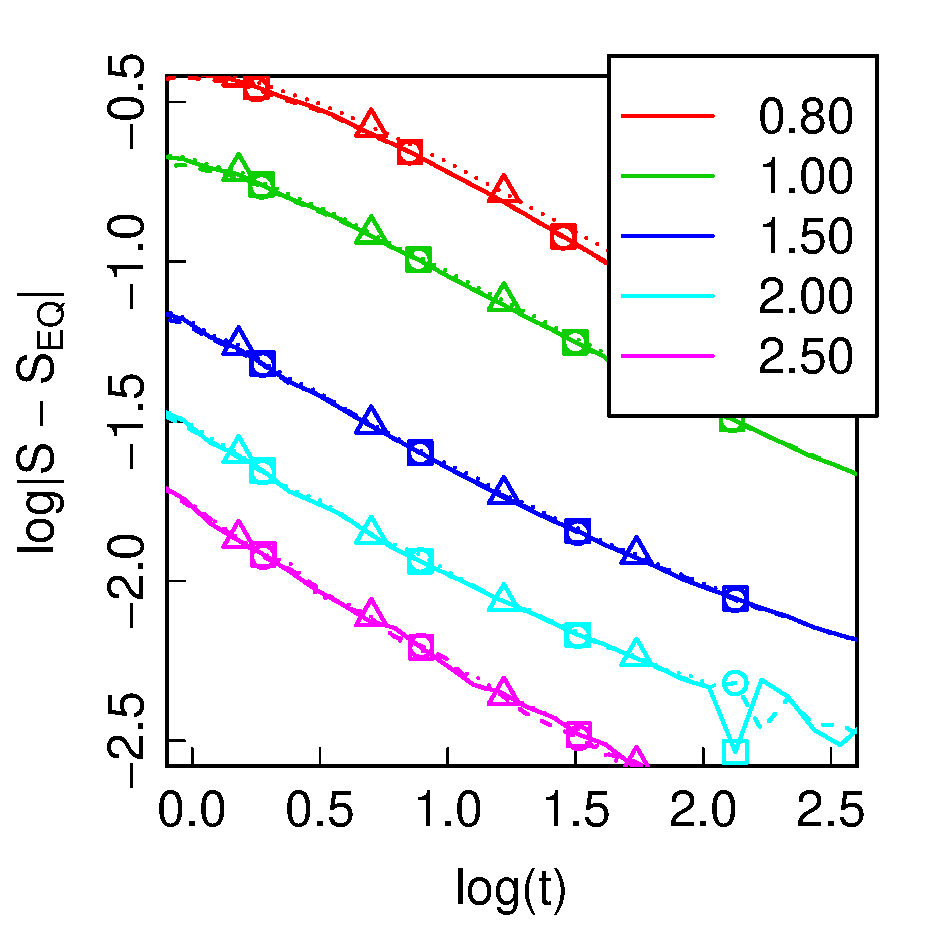
\includegraphics[width=\textwidth]{Images/relax_op_25}
\end{subfigure}
\begin{subfigure}[t]{0.7\columnwidth}
	\centering
	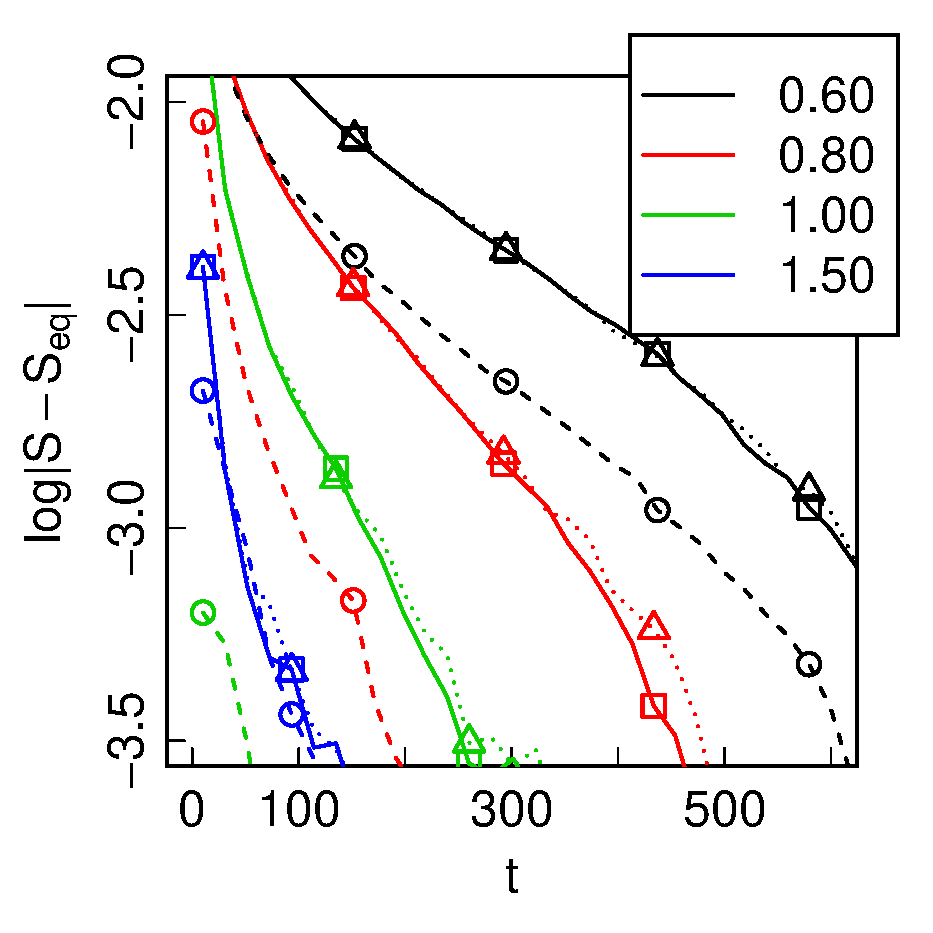
\includegraphics[width=\textwidth]{Images/relax_op_75_exp}
\end{subfigure}
	\captionsetup{width=0.9\columnwidth}
	\caption{Relaxation of order parameter to the equilibrium values for densities $\rho = (0.25, 0.75)$, left and right respectively. The squares, circles and triangles denote ``random'', ``co-aligned'' and ``counter-aligned'' initial configurations, respectively. Color indicates $k_BT$. The results are obtained on $500$ samples of $N = 6400$.}
	\label{fig:op_relaxation}
\end{figure}

To gain more insight on how the system evolves, we look into particle orientations relative to its neighbors.
Two particles are considered to be ``chained'' if 
\begin{equation}
\label{eq:chains_definition}
\begin{cases}
	|z_i - z_j| \leq d \\
	\theta_{i, j} \leq \alpha \text{ \textbf{or} } \theta_{i, j} \geq \pi - \alpha
\end{cases}
\end{equation}
where $d$ is a predefined separation distance after which particles are ``unchained'', and second condition considers only particles that are oriented along the same direction, within a certain angle $\alpha$. We define one to be ``right'' chain if all the particles satisfy $\theta_i \leq \alpha$, ``left'' if $\theta_i \geq \pi - \alpha$, and ``undefined'' in all other cases. Then we can measure the probability of two neighbouring chains to be ``left-left'' (``LL'') or ``left-right'' (``LR''), etc. The ``undefined'' chains can consist only of solitary particles, and so we suggest to treat all particles as separate chains (i.e. $d \ll D$)

The main results are shown at the Fig.~\ref{fig:prob_relaxation}.

First of all, we need to note that due to the symmetry of the system potential, the equilibrium results for the pairs ``LL'' -- ``RR'' and ``LR'' -- ``RL'' are the same, accounting for the statistical error.

Similar to order parameter, for the low density the relaxation for any of the given orientation pairs suggests power law behavior. Also is important that there is little difference in slope for co-aligned and counter-aligned orientation pairs, as well as little influence of the $k_BT$. The respective pairs (``LL'' -- ``RR'' and ``LR'' -- ``RL'') quickly relax to the same values and then the relaxation follows the same path.

For the high density the behavior is more complicated. First of all, the results suggest the exponential relaxation for prevalent (in this case ``RR'') orientation pair, with the power strongly dependent on the $k_BT$. On the other hand, the minority orientation pair (``LL'') relaxes differently after the initial moments and before the relaxation to the same values. We can see that most clearly for the $k_BT = 2.5$ in the $t \in (5, 15)$ range.

Another observation is that co-aligned orientation pairs relaxes slower then counter-aligned. It can be attributed to less favorable energy configuration of the latter, and therefore much lesser representation on the equilibrium.

\begin{figure}[t]
\centering
\begin{subfigure}[t]{0.49\columnwidth}
	\centering
	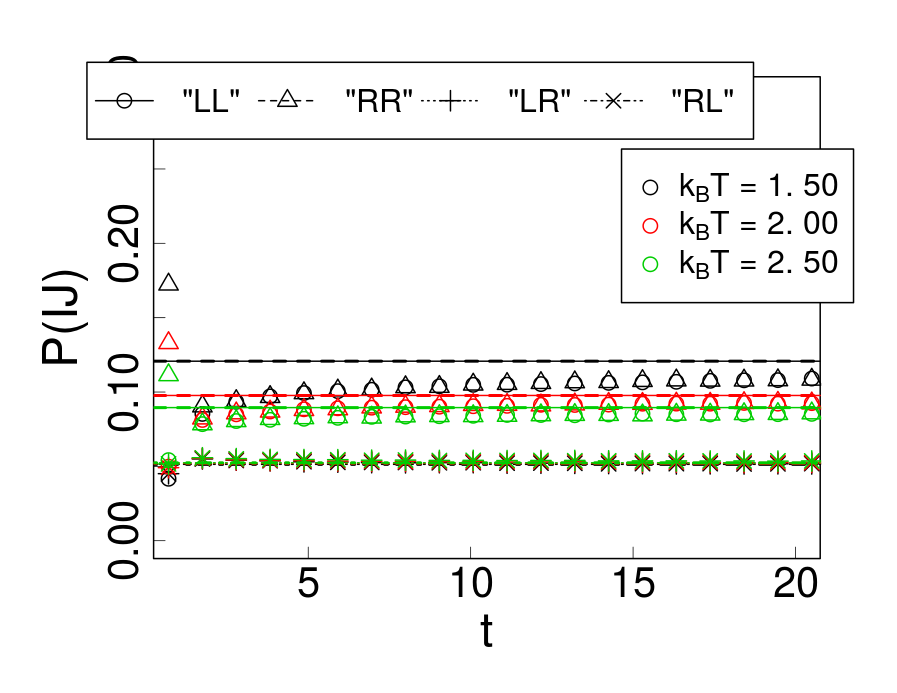
\includegraphics[width=\textwidth]{Images/Particle_probs_25}
\end{subfigure}
\begin{subfigure}[t]{0.49\columnwidth}
	\centering
	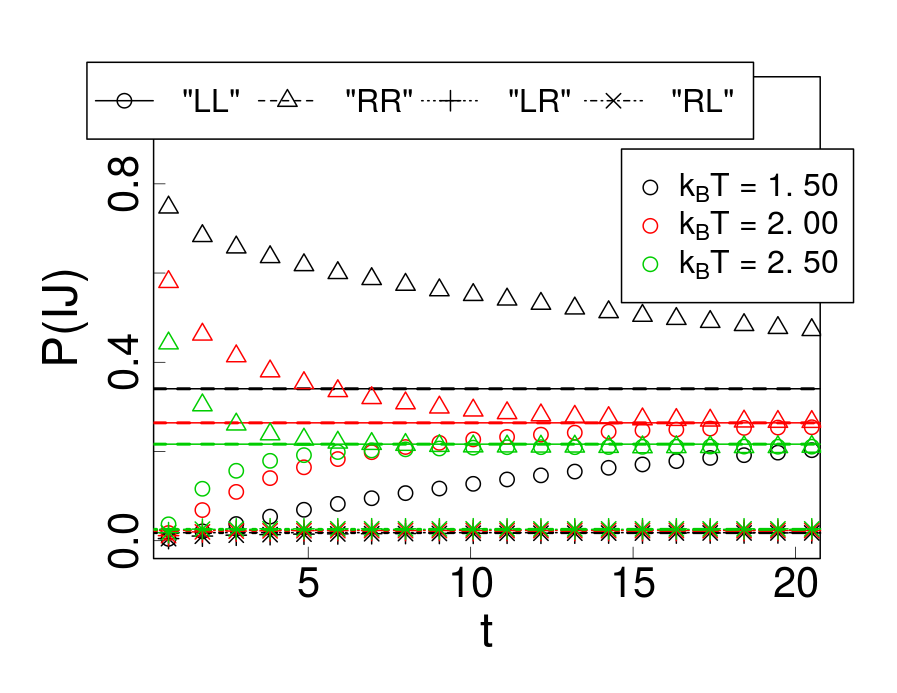
\includegraphics[width=\textwidth]{Images/Particle_probs_75}
\end{subfigure}

\begin{subfigure}[t]{0.49\columnwidth}
	\centering
	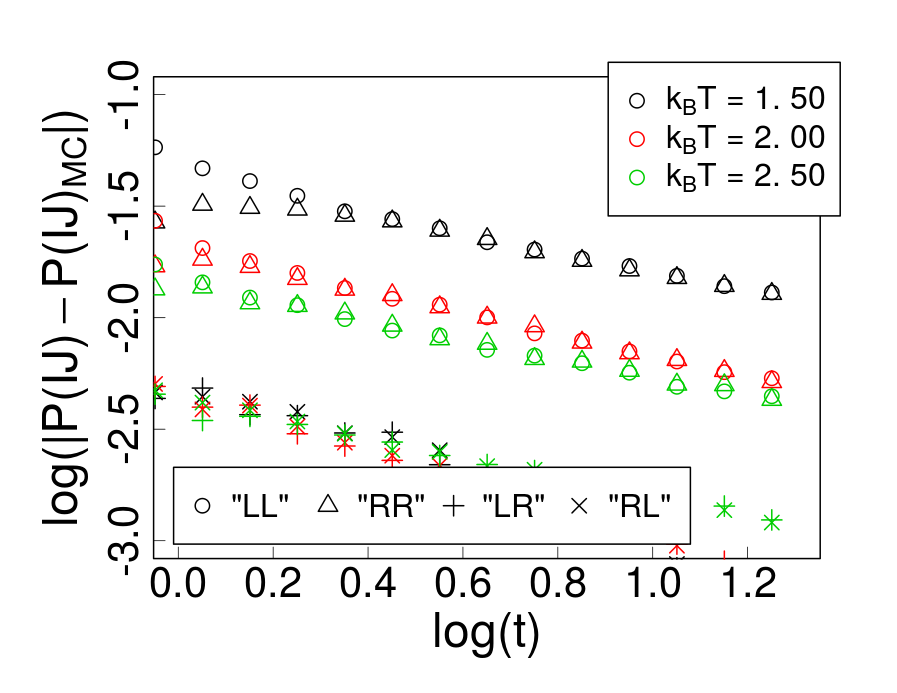
\includegraphics[width=\textwidth]{Images/Particle_probs_relaxation_25}
\end{subfigure}
\begin{subfigure}[t]{0.49\columnwidth}
	\centering
	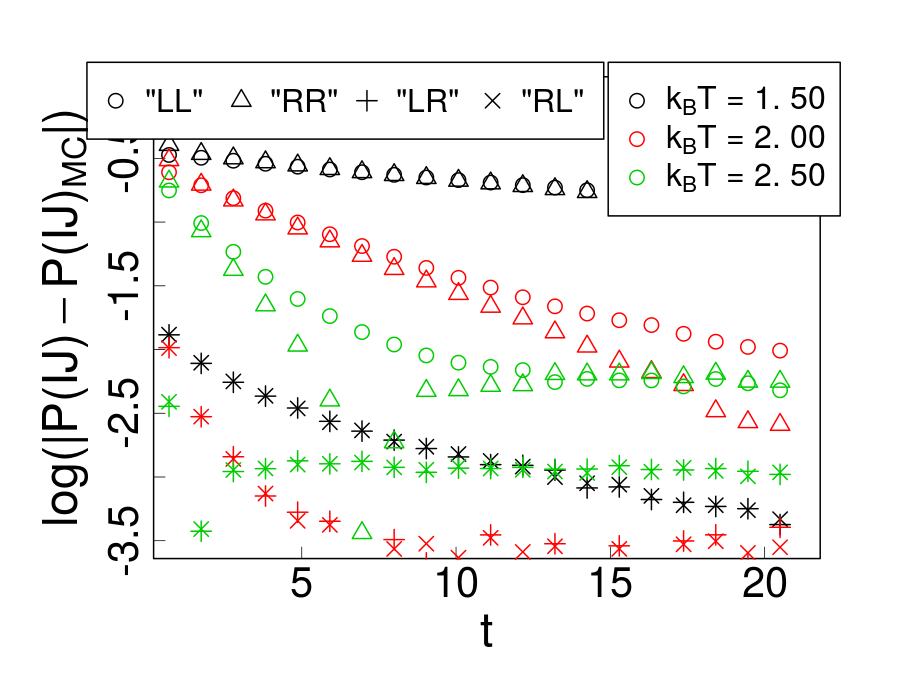
\includegraphics[width=\textwidth]{Images/Particle_probs_relaxation_75}
\end{subfigure}
	\captionsetup{justification=centering, width=0.9\columnwidth}
	\caption{Relative particle orientation probabilities (top) and their relaxation to the equilibrium values (bottom), for low ($\rho = 0.25$) and high ($\rho = 0.75$) density at the left and right respectively. Lines show the equilibrium results, however, the pairs ``LL'' -- ``RR'' and ``LR'' -- ``RL'' values are indistinguishable at this scale. The simulations start from co-aligned initial configuration.}
	\label{fig:prob_relaxation}
\end{figure}

To check if simulations are loosing memory of initial configuration, we measure autocorrelation function of a particle orientation:
\begin{equation}
\label{eq:autocorrelation_ld}
	C(t) = \langle\cos\theta_i(t) \cdot \cos\theta_i(0)\rangle
\end{equation}
here $\theta_i(0)$ is the orientation of a particle $i$ at the beginning of simulation and $\theta_i(t)$ is the orientation of the same particle in the same sample at the time $t$. The ensemble-averaging is done over all particles.

The main results are presented at the Fig.~\ref{fig:autocorrelation}. The results clearly shows the exponential tail for any given combination of parameters. However for short time scale the behavior isn't exponential, although in that case the relaxation is faster than the exponential regime, as we can clearly see in case of $k_BT = 0.8$ and $\rho = 0.25$ at the left of Fig.~\ref{fig:autocorrelation}. The relaxation time steadily increases with $k_BT$. Additionally we want to note that ``random'' initial configuration de-correlates faster than ``co-aligned'', albeit slower than ``counter-aligned'' configurations.

\begin{figure}[t]
	\begin{subfigure}[t]{0.42\columnwidth}
		\centering
		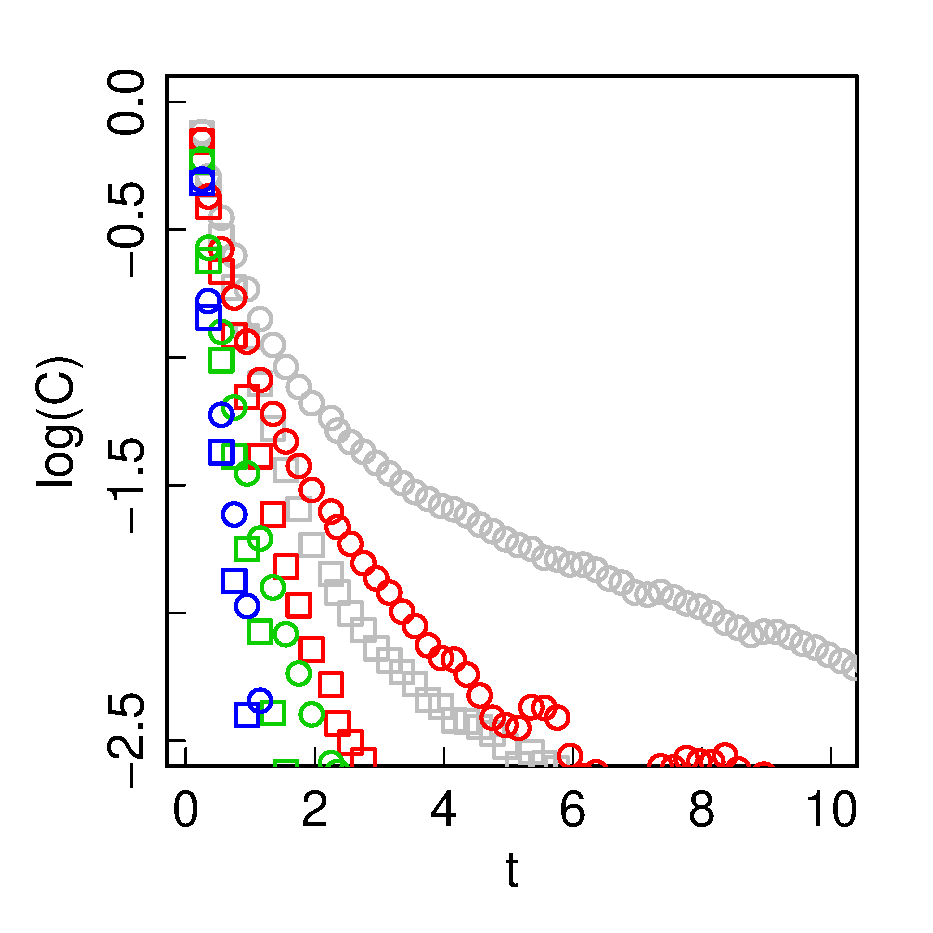
\includegraphics[width=\textwidth]{Images/Autocors_25}
	\end{subfigure}
	\begin{subfigure}[t]{0.49\columnwidth}
		\centering
		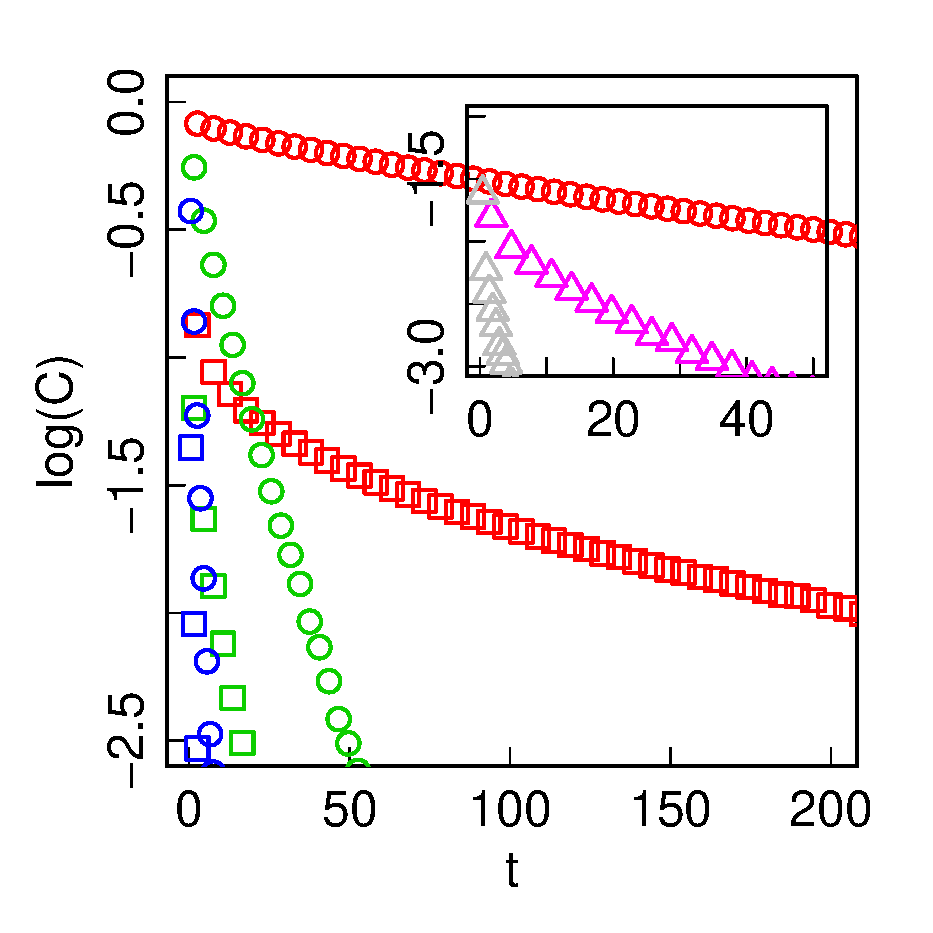
\includegraphics[width=\textwidth]{Images/Autocors_75}
	\end{subfigure}
	\captionsetup{justification=centering, width=0.9\columnwidth}
	\caption{Autocorrelation of particles orientation as function of time for LD simulations. The squares, circles and triangles denote ``random'', ``co-aligned'' and ``counter-aligned'' initial configurations, respectively. The color codes $k_BT$ values. The results are obtained on $500$ samples of $N = 6400$.}
	\label{fig:autocorrelation}
\end{figure}


